\documentclass[12pt,twoside]{article}
\usepackage[dvipsnames]{xcolor}
\usepackage{tikz,graphicx,amsmath,amsfonts,amscd,amssymb,bm,cite,epsfig,epsf,url}
\usepackage[hang,flushmargin]{footmisc}
\usepackage[colorlinks=true,urlcolor=blue,citecolor=blue]{hyperref}
\usepackage{amsthm,multirow,wasysym,appendix}
\usepackage{array,subcaption} 
% \usepackage[small,bf]{caption}
\newcommand{\red}[1]{{\leavevmode\color{red}{#1}}}
\newcommand{\blue}[1]{{\leavevmode\color{blue}{#1}}}
\usepackage{enumitem}


\makeatletter
\renewcommand*\env@matrix[1][*\c@MaxMatrixCols c]{%
  \hskip -\arraycolsep
  \let\@ifnextchar\new@ifnextchar
  \array{#1}}
\makeatother

\begin{document}

\begin{center}
{\large{\textbf{Homework 8}} } \vspace{0.2cm}\\
Due October 16thth at 12 am
\\
\end{center}
\begin{enumerate}[label=8.1]
\item A
\begin{itemize}
    \item notice that $\Tilde{U}\Tilde{\Sigma}\Tilde{V^t}_{i,j}=\sigma_{k=1}^{r}U_{i,k}V_{k,j}\simga_{k}$ 
    \item and $U\Sigma V^T=\sigma_{k=1}^{n}U_{i,k}V_{k,j}\simga_{k}=\sigma_{k=1}^{r}U_{i,k}V_{k,j}\simga_{k}+0=\Tilde{U}\Tilde{\Sigma}\Tilde{V^t}_{i,j}$ thus the iquality holds. 
\end{itemize}
\item B
\begin{itemize}
    \item the vectors $v_{r+1}...v{m}$ form an orthonormal basis for the kernel of A. 
    \item notice first that V is an orthogon matrix so its colomns already meet orthomonality requirments 
    \item further note that for any i$\in[r+1,m]$ we have $Av_i=\sigma_iu_i=0u_i=0$ implying that $v_i\in ker(A)$
    \item further by rank nulity therome we have $dim(ker(A))=m-rank(A)=m-r$, and as $v_{r+1}...v{m}$ are m-r liniarly independint vectors in ker(A) they form a basis for ker(A)
\end{itemize}
\item C
\begin{itemize}
    \item consider the set of vectors $\{u_1..u_r\}$ as these are columns of an orthogonal matrix they are orthonomral. 
    \item furhter we know that $dim(im[g(A))=rank(A)$ and that a vector $y\in \mathbb{r}^n$ is included in the image of A if there exists a vector $x\in \mathbb{R}^m$ such that $AX=y$ and we know that $\forall i\in[1,r] Av_i=\simga_iu_i$ thus $\{u_1..u_r\}\in im(A)$ and as they are r orthonormal linearly independent  vectors that are all in a subspace of dimension R they span teh space and are thus an orthonomormal basis for image of A
\end{itemize}
   \end{enumerate}
   
   
   \begin{enumerate}[label=8.2]
 \item a 
   \begin{itemize}
         \item we know that $\mathcal{H}(1)=A^1=A$ by definition of an adjacency matrix, $A_{i.j}$ takes a value of 1, if there is an edge between vertex i and j, an edge can be understood as a path of length one, thus $A_{i,j}$ encodes the number of paths of length one between vertex i and j. 
   \end{itemize}
   \item B
   \begin{itemize}
       \item suppose that this property holds up to some $k-1\geq 1$ that is $\mathcal{H}(k-1)_{i,j}$ represents the number of paths of length k-1 between vertex i and j. 
       \item we can see that $\mathcal{H}(k)_{i,j}=\Simga_{l=1}^{n}{H}(k)_{i,l}A_{l,j}$ where ${H}(k)_{i,l}$ can be thought of as the number of paths of length k-1 between vertex i and l, and $A_{l,j}$ is a binary varible representing if there is an edge (or path of length 1) between vertex l and j. thus $\mathcal{H}(k)_{i,j}=\Simga_{l=1}^{n}{H}(k)_{i,l}A_{l,j}$ can be thought of as the sum of the number of paths of length k-1 from i to adjacent vertices of J or in other words the number of paths of length k from i to j.  
   \end{itemize}
   \item C
   \begin{itemize}   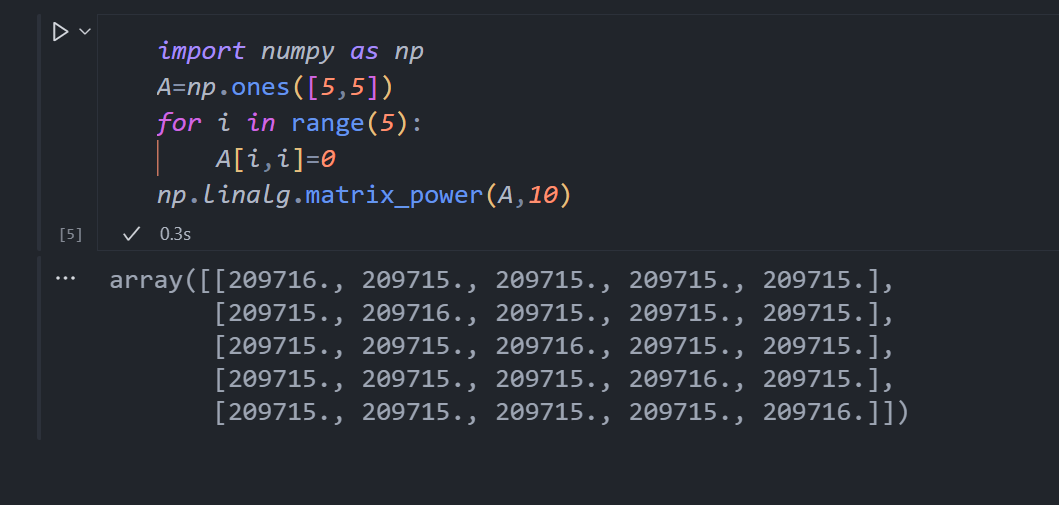
\includegraphics[width=12cm]{homework 8/homework 8 question 3.PNG}
   \item as one can see from the output of the above code there are 209716 paths of length 10 between any nodes $i\neq j$ i the graph and 209715 paths of length 10 from a node to its self in the graph 
 \end{itemize}

   \end{enumerate}
\end{document}
